% !TEX program = xelatex

\documentclass[b5paper, 11pt, openleft]{memoir}

\usepackage{indentfirst}

%%% Font setup
\usepackage[no-math]{fontspec}
\setmainfont{Zilla Slab}
\setmonofont[Scale = MatchLowercase]{Iosevka Custom}
\XeTeXlinebreaklocale="en_EN"
\XeTeXlinebreakskip=0pt plus 3pt
\emergencystretch=1em

\usepackage{mathtools}
\usepackage[math-style = ISO, mathrm = sym, warnings-off = {mathtools-colon}]{unicode-math}
\setmathfont[Scale = MatchLowercase]{Concrete-Math.otf}
\noDisplayskipStretch
\setoperatorfont\symscr
\everymath{\displaystyle}

%%% Stylings
% Page Layout and Margins
\setsecnumdepth{subsection}
\settocdepth{subsection}
\setlrmarginsandblock{4cm}{1.5cm}{*}
\setulmarginsandblock{3cm}{2.5cm}{*}
\setlength{\headheight}{30pt}
\setlength{\parindent}{1.5cm}
\setlength{\parskip}{0.3em}
\setlength{\beforechapskip}{20pt}
\renewcommand{\arraystretch}{1}
\allowdisplaybreaks
\setSpacing{1.5}
\checkandfixthelayout

% Footnotes
\usepackage{fancyhdr}
\pagestyle{fancy}
\fancyhead[LE]{\textbf{\thepage ~ $\big\vert$ \leftmark}}
\fancyhead[RO]{\textbf{\rightmark ~ $\big\vert$ \thepage}}
\fancyhead[RE, LO, C]{}

% Styling Figures
\usepackage{multicol, caption}
\setlength{\columnseprule}{1pt}
\def\columnseprulecolor{\color{lightgray}}
\DeclareCaptionLabelSeparator{pipe}{ $\vert$ }
\captionsetup{
    labelfont = {bf},
    font = {small, sc},
    width = 0.6\textwidth,
    labelsep = pipe,
    figurename = \textbf{Fig. }
}

% Styling Titles
\renewcommand{\partnamefont}{\LARGE\bfseries\scshape\centering}
\renewcommand{\partnumfont}{\LARGE\bfseries\scshape\centering\MakeUppercase}
\renewcommand{\midpartskip}{\par\rule{1in}{0.5pt}\vspace{1em}\par}
\renewcommand{\printparttitle}{\HUGE\bfseries\scshape\centering}
\renewcommand{\afterpartskip}{\relax}
\chapterstyle{veelo}
    \renewcommand*{\printchapternum}{%
    \makebox[0pt][l]{%
    \hspace{.8em}%
    \resizebox{!}{\beforechapskip}%
    {\chapnumfont \thechapter}%
    \hspace{.8em}%
    \rule{2\midchapskip}{\beforechapskip}%
    }%
}

% Packages
\usepackage[dvipsnames]{xcolor}
\usepackage{subcaption, graphicx, pdfpages, float, wrapfig}
\usepackage{minted}
\usemintedstyle{algol_nu}
\setminted{
    frame = lines,
    bgcolor = lightgray,
    linenos,
	breaklines
}
\usepackage{csquotes}
\graphicspath{{figures/}}
\usepackage[inline]{enumitem}

\usepackage[colorlinks, allcolors = blue]{hyperref}
\usepackage{cleveref}

%%% Mathematical packages 
\usepackage[]{siunitx}
\usepackage{physics2}
\usepackage{derivative}
\usephysicsmodule{ab, ab.braket, nabla.legacy, op.legacy}
\usephysicsmodule{ab.legacy}
\usepackage[makeroom]{cancel}
% Proofs
\usepackage{amsthm}
\usepackage{tcolorbox}
\tcbuselibrary{breakable, theorems, skins}
\newtcbtheorem[auto counter, crefname = {theorem}{theorems}, Crefname = {Theorem}{Theorems}]{theorem}{Theorem}{
    coltitle = black,
    sharp corners, frame hidden, enhanced, colback = lightgray!10, breakable,
    borderline west = {3pt}{-3pt}{lightgray},
    detach title = true,
    fonttitle = \bfseries, before upper = {\tcbtitle\quad}
}{theorem}
\newtcbtheorem[auto counter, crefname = {axiom}{axioms}, Crefname = {Axiom}{Axioms}]{axiom}{Axiom}{
    sharp corners, colback = lightgray!40, colframe = darkgray, breakable
}{axiom}
\newtcbtheorem[auto counter, crefname = {definition}{definition}, Crefname = {Definition}{Definition}]{df}{Definition}{
    sharp corners, colback = lightgray!40, colframe = darkgray, breakable
}{df}
\newtcbtheorem[auto counter, number within = section]{exmp}{Example}{
    colback = lightgray!40, colframe = darkgray, breakable
}{exmp}
\newtcbtheorem[auto counter, number within = chapter, crefname = {remarks of chapter }{remarks of chapter }, Crefname = {Remarks}{Remarks}]{remark}{Remarks on chapter }{
    colback = lightgray!10, colframe = black, breakable
}{remark}

%%% Mathematical commands
% Geometry
\let\line\overline
% Mathematical constants
\newcommand{\e}{\symrm{e}}
\newcommand{\im}{\symrm{i}}
\newcommand{\cpi}{\symrm{\pi}}
\DeclareMathOperator*{\ssum}{\symrm{\Sigma}}
\DeclareMathOperator*{\Proj}{\symrm{Proj}}
\DeclareMathOperator*{\sgn}{\symrm{sgn}}
% Vector notations
\newcommand{\vv}[1]{\pmb{\symrm{#1}}}
\newcommand{\vdot}{\pmb{\cdot}}
\newcommand{\conj}{^{\ast}}
\newcommand{\dagr}{^{\dag}}
\newcommand{\trnsp}{^{\intercal}}
\newcommand{\iden}{\symbb{I}}
\newcommand{\uv}[1]{\hat{\vv{e}}_{#1}}
\newcommand{\tensor}{\otimes}
\newcommand{\bmat}[1]{
	\begin{bmatrix}
		#1
	\end{bmatrix}
}
\newcommand{\ihat}{\hat{\i}}
\newcommand{\jhat}{\hat{\j}}
\newcommand{\khat}{\hat{k}}
\newcommand{\xhat}{\hat{\vv{x}}}
\newcommand{\yhat}{\hat{\vv{y}}}
\newcommand{\zhat}{\hat{\vv{z}}}
\newcommand{\rhat}{\hat{\vv{r}}}
\newcommand{\nhat}{\hat{\vv{n}}}
\newcommand{\that}{\hat{\vv{\theta}}}
\newcommand{\phat}{\hat{\vv{\rho}}}
\newcommand{\eflux}{\symrm{\Phi}_E}
\newcommand{\mflux}{\symrm{\Phi}_B}
\newcommand{\sint}{\int_{\mathcal{S}}}
\newcommand{\aint}{\int_{\mathcal{A}}}
\newcommand{\vint}{\int_{\mathcal{V}}}
\newcommand{\cint}{\int_{\mathcal{C}}}
\newcommand{\bperm}{\symrm{\mu}_0}
\newcommand{\eperm}{\symrm{\varepsilon}_0}
\newcommand{\rc}{{{\mbox{$\resizebox{1.2ex}{1.15ex}{
\includegraphics[trim= 1em 0 14em 0,clip]{fonts/scriptr.pdf}}$}}}}
\newcommand{\brc}{{{\mbox{$\resizebox{1.2ex}{1.15ex}{
\includegraphics[trim= 1em 0 14em 0,clip]{fonts/boldcursiver.pdf}}$}}}}
\newcommand{\rchat}{{{\mbox{$\hat\rcurs$}}}}
\newcommand{\peval}[1]{\left(\left.#1\right.\right\rvert}
% Differences
\DeclareMathOperator{\kdel}{\symrm{\delta}}
\DeclareMathOperator{\ddel}{\symrm{\delta}}
\newcommand{\Dd}{\symrm{\Delta}}
% Physics quantities symbols
\newcommand{\lagr}{\mathcal{L}}
\newcommand{\haml}{\mathcal{H}}
\newcommand{\hilb}{\mathcal{E}}
\newcommand{\emf}{\mathcal{E}}
% Calculus notations
\newcommand{\appr}{\rightarrow}
\newcommand{\alc}[2][0.3]{&\parbox[c]{#1\textwidth}{#2}}
\newcommand{\pintm}[1]{\mathcal{D}[#1]}
% Mathematical conjunctions and expressions
\newcommand{\mathand}{\quad\textrm{and,}\quad}
\newcommand{\mathor}{\quad\textrm{or,}\quad}
\newcommand{\mathif}{\quad\textrm{if}\quad}
\newcommand{\mathiff}{\quad\textrm{\emph{iff}}\quad}
\newcommand{\maththerefore}{\therefore\emquad}
\newcommand{\ifft}{\emph{iff}}
% Notational commands
\newcommand{\flatfrac}[2]{#1\fracslash#2}
% Column types
\newcolumntype{C}{>{$}c<{$}}
\newcolumntype{L}{>{$}l<{$}}
\newcolumntype{R}{>{$}r<{$}}

%%% Type commands
\newcommand{\conclusion}{\section{Conclusion for Chapter \thechapter}}
\newcommand{\formula}{\section{Formula from Chapter \thechapter}}
\newcommand{\prelude}[1]{
    \chapter*{Prelude: #1}
    \addcontentsline{toc}{chapter}{Prelude: #1}
}
\newcommand{\prerequisites}[1]{\textbf{Prerequisites:}~\emph{#1}}

% Bibliographies
\usepackage[
    backend = biber,
    style = phys,
    sorting = anyvt
]{biblatex}
\addbibresource{bibfile.bib}

\usepackage[inkscapeversion = 1, inkscapelatex = true]{svg}
\svgpath{{code/}}
% Indices
% \usepackage{imakeidx}
% \makeindex

\begin{document}

\frontmatter
\title{
	\vspace{-5em}
	\textbf{
		Experiment on\\
		\enquote{Measurement of gravity by the voltage difference induced on a solenoid by a free falling magnet}
	}
}
\author{Puripat Thumbanthu}
\date{Started: 17/09/2024, Revision: \today}
\maketitle

\vspace{-7em}
\tableofcontents*

\mainmatter

\chapter{Introduction}

One of the dream that most physics student pursue is to be able to measure the Earth's gravitational acceleration from every physical quantities accessible, whether it would be the period of a pendulum, the surface tension of water, the timing of a ball bearing, etc. I also share that dream; thus, I choose to measure Earth's gravitational acceleration using electromagnetic induction.

As we shall see in \cref{sec:related-works}, there already has been multiple times when these form of experiments have been conducted. But they require quite a complicated setup. So in this work, I challenge myself to work with the most basic setup there is: a magnet, a single solenoid, and an oscilloscope.

\paragraph{Hypothesis} It is possible to measure the Earth's gravitational constant using electromagnetic induction.

\paragraph{Objectives} To measure the Earth's gravitational constant using electromagnetic induction in the simplest way possible.

\chapter{Literature reviews}

\section{Problem statement}
\label{sec:problem-statement}

The problem is as follows: consider a solenoid of length $L$, radius $R$, made from copper wire with resistivity $\Omega$, wound into $K$ layers, each consisting of $N$ loops. A free-falling Amperian magnet of length $\mathcal{l}$, mass $M$, and magnetic dipole moment $\mu$ is dropped from a height $z_0$ through the center of the solenoid. From the induced electromotive force $\emf$, is possible to determine Earth's gravitational constant by analyzing the voltage difference alone?

To solve this problem, the first step is to calculate the magnetic flux, $\mflux$, through the solenoid. Once the flux is known, the induced current and electromotive force, which are all functions of the magnet's position and velocity, can be determined. With the induced current, Lenz's law determines the force acting on the magnet. Finally, Newton's law is applied to combine this force with Earth's gravitational force into a differential equation that describes the magnet's position and velocity.

Since the magnet's velocity is a function of gravity, and the voltage is a function of velocity, Earth's gravity can be directly determined by measuring the voltage. However, the data is complex to process, so we focus on the minima of the voltage, which can be directly measured using an oscilloscope. By fitting this minimum voltage to the expected function, we can accurately calculate the gravitational force.

However, we will see in \cref{sec:perfect-magnetic-dipole} that the force contribution from Lenz's law makes the problem in its full form is not analytically solvable. Therefore, some simplifications must be made for an analytical solution to be viable.

\section{Related works}
\label{sec:related-works}

From my current knowledge, three studies have addressed the measurement of Earth's gravitational acceleration via electromagnetic induction. \emph{Ahmad Khan, Amar} \lcite{khan-no-date} has conducted a similar experiment but relied on numerical solutions of the entire voltage function without the effect from Lenz's law. \emph{Riad, Ihaf F.} \lcite{riad-2023} had performed a comparable experiment but with multiple solenoids to capture the difference in time between each coil's induction, with a long tube guiding the magnet's descent. Lastly, \emph{Jing, Liu} \lcite{jing-2019} succeeded to measure Earth's gravitational acceleration by using two solenoids that functions like a traditional photogate. However, none of these studies have included the magnet's retardation effect from Lenz's law yet.

\section{Simplification of problem}

The problem is simplified as follows: the finite-length solenoid is replaced with a solenoid with zero length, wounded around $N$ times, and the Amperian magnet is replaced by a perfect magnetic dipole with magnetic moment coefficient $\mu$. Funnily, this problem is still unsolvable analytically. So, we would have to resort to either neglection of terms or numerical methods. In this study, we've chosen not to neglect the Lenz's law, but to compare the results observed with the simulated theoretical voltage difference in order to find Earth's gravitational acceleration.

\section{Induction from a perfect magnetic dipole}
\label{sec:perfect-magnetic-dipole}

First, let's evaluate the magnetic flux on a loop. Let there be a magnet with a magnetic moment $\vv{m}$ pointing downwards ($\vv{m} = m\zhat$) situated at $z(t = 0) = h$. The magnetic flux is given by
\begin{equation}
	\mflux = \sint \vv{B}(\brc) \vdot \odif{\vv{A}}.
\end{equation}
The surface area vector element $\odif{\vv{A}}$ is defined as $\nhat\odif{A}$, where $\nhat$ is a vector normal to the surface of integration. In a cylindrical coordinate $(\rho, \theta, z)$ with the area integration element $\rho\odif{\rho}\odif{\theta}$,
\begin{equation}
	\odif{\vv{A}} = \nhat\rho\odif{\rho}\odif{\theta};
\end{equation}
hence,
\begin{equation}
	\mflux = \sint \vv{B}(\brc) \vdot \odif{\vv{A}} = \sint \vv{B}(\brc)\vdot\zhat\rho\odif{\rho}\odif{\theta}.
\end{equation}

The magnetic field, $\vv{B}$ of a perfect magnetic dipole is given by 
\begin{equation}
	\vv{B}(\brc) = \frac{\bperm}{4\cpi}\ab[\frac{3\brc(\vv{m}\vdot\brc)}{\rc^5} - \frac{\vv{m}}{\rc^3}],
\end{equation}
where $\brc$ is a vector that points from the source to any arbitrary point, $\vv{m}$, the magnetic dipole moment, and $\bperm$, the magnetic permeability. \lcite{zangwill-2013}
\begin{figure}[b]
	\centering
	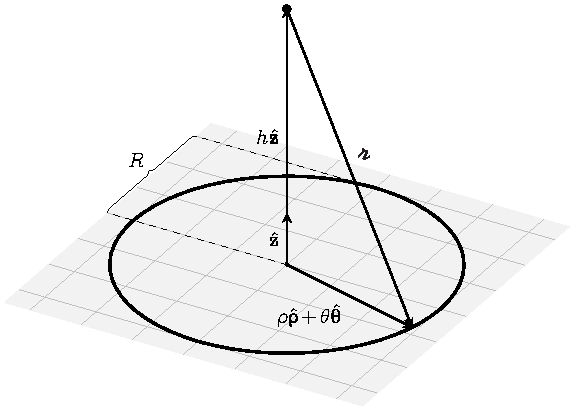
\includegraphics{perfect-dipole-over-loop.pdf}
	\caption{Perfect magnetic dipole hovering at a height $h$ over a loop radius $R$.}
	\label{fig:perfect-dipole-over-loop}
\end{figure}
Since we want to find the magnetic flux over a copper wire illustrated in \cref{fig:perfect-dipole-over-loop}, $\brc$ must be a vector that points from the magnet to any arbitrary points in the wire. Geometrically, $h\zhat + \brc = \rho\phat + \theta\that$; thus,
\begin{equation}
	\brc = \rho\phat + \theta\that - h\zhat.
\end{equation}
Using $\vv{m} = -m\zhat$,
\begin{align}
	\vv{B}(\brc) &= \frac{\bperm}{4\cpi}\ab[\frac{3\brc(-m\zhat\vdot(\rho\phat + \theta\that - h\zhat))}{\rc^5} + \frac{m\zhat}{\rc^3}] \\
				 &= \frac{\bperm}{4\cpi}\ab[\frac{3\brc}{\rc^5}(mh) + \frac{m\zhat}{\rc^3}] \\
	\vv{B}(\brc) \cdot \zhat &= \frac{\bperm}{4\cpi}\ab[\frac{3mh}{\rc^5}(\brc\vdot\zhat) + \frac{m}{\rc^3}(\zhat\vdot\zhat)] \\
							 &= \frac{\bperm}{4\cpi}\ab[\frac{1}{\rc^3} - \frac{3h^2}{\rc^5}]
\end{align}
The magnetic flux over the disk is then
\begin{align}
	\mflux &= \int\limits_{0}^{2\cpi}\int\limits_{0}^{R}\ab[\vv{B}(\brc)\cdot\zhat]\rho\odif{\rho}\odif{\theta} \\
		   &= \frac{\bperm m}{4\cpi} \int\limits_{0}^{2\cpi}\int\limits_{0}^{R}\ab(\frac{1}{\rc^3} - \frac{3h^2}{\rc^5})\rho\odif{\rho}\odif{\theta} \\
		   &= \frac{\bperm m}{4\cpi} \int_0^{2\cpi}\odif{\theta} \times \ab[
		   \int_0^{R}\frac{\rho}{(\rho^2 + h^2)^{\frac{3}{2}}}\odif{\rho} - 3h^2\int_0^R\frac{\rho}{(\rho^2 + h^2)^{\frac{5}{2}}}\odif{\rho}
		   ] \\
		   &= \frac{\bperm m}{2}\ab[\peval{-\frac{1}{(\rho^2 + h^2)^{\frac{1}{2}}}}_0^R - 3h^2\peval{ - \frac{1}{3}\times\frac{1}{(\rho^2 + h^2)^{\frac{3}{2}}}}_0^R] \\
		   &= -\frac{\bperm m}{2}\ab[-\frac{1}{(R^2 + h^2)^{\frac{1}{2}}} + \frac{1}{h} + h^2\ab(\frac{1}{(R^2 + h^2)^{\frac{3}{2}}} - \frac{1}{h^3})] \\
		   &= -\frac{\bperm m}{2}\ab[\frac{h^2}{(R^2 + h^2)^{\frac{3}{2}}} - \frac{1}{(R^2 + h^2)^{\frac{1}{2}}}]
\end{align}
The change in magnetic flux is proportional to the electromotive force, which is distributed throughout the wire. If the wire is wounded around $N$ times, the electromotive force is also multiplied by $N$. At a certain height $h$,
\begin{align}
	\emf &= -N\odv{\mflux}{t} \\
		 &= -\frac{N\bperm m}{2}\ab[\odv*{\frac{h^2}{(R^2 + h^2)^{\frac{3}{2}}}}{t} - \odv*{\frac{1}{(R^2 + h^2)^{\frac{1}{2}}}}{t}] \\
		 &= -\frac{N\bperm m}{2}\ab[\ab(\frac{2h}{(R^2 + h^2)^{\frac{3}{2}}} - \frac{3h^3}{(R^2 + h^2)^{\frac{5}{2}}})\odv{h}{t} - \frac{h}{(R^2 + h^2)^{\frac{3}{2}}}\odv{h}{t}] \\
		 &= -\frac{N\bperm mh}{2}\odv{h}{t}\ab[\frac{1}{(R^2 + h^2)^{\frac{3}{2}}} - \frac{3h^2}{(R^2 + h^2)^{\frac{5}{2}}}] \label{eq:theoretical-voltage}
\end{align}

In a wire, $\emf$ is identical to $V$, the voltage. By Ohm's law, $V = I\Omega$, the current induced by a perfect magnetic dipole falling is
\begin{align}
	I &= -\frac{N\bperm mh}{2\Omega}\odv{h}{t}\ab[\frac{1}{(R^2 + h^2)^{\frac{3}{2}}} - \frac{3h^2}{(R^2 + h^2)^{\frac{5}{2}}}].
\end{align}
The Biot-Savart law states that the magnetic field generated by a current $I$ is given by
\begin{equation}
	\vv{B}'(\brc) = \frac{\bperm}{4\cpi}\cint\frac{I\odif{\vv{l}} \times \brc'}{|\brc'|^3}\odif{\brc'}.
\end{equation}
The system that we're interested in: magnetic field directly above a ring with uniformed current distribution, has a very well-known result in electrodynamics: \lcite{griffiths-2023}
\begin{equation}
	\vv{B}(h\zhat) = \frac{\bperm I}{2}\frac{R^2}{(R^2 + z^2)^{\frac{3}{2}}}\zhat \label{eq:b-field-over-loop}
\end{equation}
We can use this result to directly evaluate the force that the ring acts on the magnetic dipole.

A magnet in an external magnetic field experiences a force that follows the direction of the external field's gradient: \lcite{boyer-1988}
\begin{equation}
	\vv{F} = \grad(\vv{m}\cdot\vv{B})
\end{equation}
where $\vv{m}$ is of the magnet that experiences the force. From \cref{eq:b-field-over-loop},
\begin{align}
	\vv{m}\cdot\vv{B} &= -m\zhat\cdot\vv{B} \\
					  &= -\frac{m\bperm I}{2}\frac{R^2}{(R^2 + z^2)^{\frac{3}{2}}},
\end{align}
and
\begin{align}
	&\grad(\vv{m}\cdot\vv{B}) \nonumber\\
	&= \ab[\xhat\pdv{}{x} + \yhat\pdv{}{y} + \zhat\pdv{}{z}]\ab(-\frac{m\bperm I}{2}\frac{R^2}{(R^2 + z^2)^{\frac{3}{2}}}) \\
	&= \zhat\pdv*{\ab(-\frac{m\bperm I}{2}\frac{R^2}{(R^2 + z^2)^{\frac{3}{2}}})}{z} \\
	&= -\frac{m\bperm}{2}\pdv*{\ab(-\frac{N\bperm mz}{2\Omega}\odv{z}{t}\ab[\frac{1}{(R^2 + z^2)^{\frac{3}{2}}} - \frac{3z^2}{(R^2 + z^2)^{\frac{5}{2}}}]\frac{R^2}{(R^2 + z^2)^{\frac{3}{2}}})}{z}\zhat \nonumber\\
	&= \ab(\frac{m\bperm}{2})^2\frac{NR^2}{\Omega}\odv{z}{t}\odv*{\ab(\frac{1}{(R^2 + z^2)^{3}} - \frac{3z^2}{(R^2 + z^2)^4})}{z} \\
	&= \frac{NR^2}{\Omega}\ab(\frac{m\bperm}{2})^2\ab(\frac{24z^3}{(R^2 + z^2)^5} + \frac{12z}{(R^2 + z^2)^4})\odv{z}{t}
\end{align}
The term $\odv{z}{t}$ must be obtained via Newton's second law. Let $M$ be the mass of the magnet, then
\begin{align}
	\vv{F} &= M\odv[ord = 2]{z}{t} \\
	M\odv[ord = 2]{z}{t} &= \ab(\frac{m\bperm}{2})^2\frac{NR^2}{\Omega}\ab(\frac{24z^3}{(R^2 + z^2)^5} + \frac{12z}{(R^2 + z^2)^4})\odv{z}{t} - Mg \\
	\odv[ord = 2]{z}{t} &= \ab(\frac{m\bperm}{2})^2\frac{12NR}{\Omega M}\ab(\frac{2z^3}{(R^2 + z^2)^5} + \frac{z}{(R^2 + z^2)^4})\odv{z}{t} - g
\end{align}
I shall let
\begin{gather}
	\alpha \equiv \ab(\frac{m\bperm}{2})^2\frac{12NR}{\Omega M}, \\
	f(z) \equiv \frac{2z^3}{(R^2 + z^2)^5} + \frac{z}{(R^2 + z^2)^4};
\end{gather}
therefore,
\begin{equation}
	\ddot{z} = \alpha f(z)\dot{z} - g
\end{equation}
By using the chain rule, the differential equation can be reduced into a first-order nonlinear ordinary differential equation.
\begin{align}
	\odv[ord = 2]{z}{t} &= \alpha f(z)\dot{z} - g \\
	\odv{\dot{z}}{z}\odv{z}{t} &= \alpha f(z)\dot{z} - g \\
	\dot{z}\odv{\dot{z}}{z} &= \alpha f(z)\dot{z} - g.
\end{align}
This is the Abel's equation of the second form, which unfortunately has no analytical solution in this case. Therefore, some terms must be neglected or approximated.

\section{Neglection of the Lenz's law}

The term $\alpha$ has a magnitude of around $10^{-20}$, which is merely impossible to detect. Therefore, one could say that if a solenoid is lengthless, it's almost impossible to detect the contribution from the Lenz's law. If that's neglected, the differential equation reads
\begin{equation}
	\ddot{z} = -g,
\end{equation}
which has a pretty well known result in classical mechanics:
\begin{gather}
	\dot{z} = v_0 - gt, \\
	z = z_0 + v_0t - \frac{1}{2}gt^2,
\end{gather}
where $v_0$ is the initial velocity and $z_0$, the initial height. Since we're dropping the magnet from zero velocity,
\begin{equation}
	\dot{z} = -gt \mathand z = z_0 - \frac{1}{2}gt^2. \label{eq:lenz-law-neglection-zzdot}
\end{equation}

As said in \cref{sec:problem-statement}, we're interested in measuring the difference between the maxima and the minima of the voltage. When the contribution from Lenz's law is neglected, we can directly substitute \cref{eq:lenz-law-neglection-zzdot} into the voltage equation \cref{eq:theoretical-voltage}, (repeated for ease of reading)
\begin{equation*}
	\emf = -\frac{N\bperm mz}{2}\odv{z}{t}\ab[\frac{1}{(R^2 + z^2)^{\frac{3}{2}}} - \frac{3z^2}{(R^2 + z^2)^{\frac{5}{2}}}]
\end{equation*}
to get\footnote{Courtesy the \texttt{SymPy} package in \texttt{Python} language for letting me evaluate these without a hassle.}
\begin{align}
	\emf &\approx \begin{multlined}[t]
		 -\frac{N\bperm m(z_0 - \frac{1}{2}gt^2)}{2}(-gt) \times \\ 
		\ab[\frac{1}{\ab(R^2 + \ab(z_0 - \frac{1}{2}gt^2)^2)^{\frac{3}{2}}} - \frac{3h^2}{\ab(R^2 + \ab(z_0 - \frac{1}{2}gt^2)^2)^{\frac{5}{2}}}]
	\end{multlined} \\
		 &= -4N\bperm gmt \frac{\ab(2R^2 - \ab(gt^2 - 2z_0)^2)\ab(gt^2 - 2z_0)}{\ab(4R^2 + \ab(gt^2 - 2z_0)^2)^{\frac{5}{2}}}
\end{align}
The next step is to take the derivative of the electromotive force w.r.t. time and find the position in which this derivative equals zero. Since we're only interested in $\odv{\emf}{t} = 0$, the actual derivative isn't required. The derivative of each function that makes up $\emf$ is already enough to do so.

Let
\begin{gather}
	f_1 \equiv t(gt^2 - 2z_0), \quad \odv{f_1}{t} = 3gt^2 - 2z_0, \\
	f_2 \equiv 2R^2 - (gt^2 - 2z_0)^2, \quad \odv{f_2}{t} = -4gt(gt^2 - 2z_0), \\
	f_3 \equiv \ab(4R^2 + \ab(gt^2 - 2z_0)^2)^{-\frac{5}{2}}, \quad \odv{f_3}{t} = -\frac{10gt(gt^2 - 2z_0)}{\ab(4R^2 + (gt^2 - 2z_0)^2)^{\frac{7}{2}}} .
\end{gather}
The product rule for three functions says
\begin{equation}
	\odv*{(f_1f_2f_3)}{t} = f_1f_2f_3\ab(\frac{1}{f_1}\odv{f_1}{t} + \frac{1}{f_2}\odv{f_2}{t} + \frac{1}{f_3}\odv{f_3}{t})
\end{equation}
For this derivative to be zero, either $f_1$, $f_2$, $f_3$, or $\textstyle\ab(\frac{1}{f_1}\odv{f_1}{t} + \frac{1}{f_2}\odv{f_2}{t} + \frac{1}{f_3}\odv{f_3}{t})$ must be zero. However, when $f_1$, $f_2$ and $f_3$, are zero, it also represents the root of $\emf$, which doesn't have zero derivative. Therefore, we're only interested in the case where $\textstyle\ab(\frac{1}{f_1}\odv{f_1}{t} + \frac{1}{f_2}\odv{f_2}{t} + \frac{1}{f_3}\odv{f_3}{t})$ is zero.

Funnily enough, the equation
\begin{equation}
	\begin{multlined}
		0 = f_1f_2f_3\ab(\frac{1}{f_1}\odv{f_1}{t} + \frac{1}{f_2}\odv{f_2}{t} + \frac{1}{f_3}\odv{f_3}{t}) = \\
		-\frac{10gt(gt^2 - 2z_0)}{4R^2 + (gt^2 - 2z_0)^2} - \frac{4gt(gt^2 - 2z_0)}{2R^2 - (gt^2 - 2z_0)^2} + \frac{3gt^2 - 2z_0}{t(gt^2 - 2z_0)}
	\end{multlined}
\end{equation}
also doesn't have any analytical solution for $t$. Therefore, we resort to numerical methods, shown in \cref{sec:data-analysis}


\chapter{Methodology}

\section{Materials}

\begin{enumerate}
	\item Cylindrical neodymium magnet (Shown in \cref{fig:magnets}, Diameter: $\qty{1}{\centi\meter}$, Height: $\qty{1.5}{\centi\meter}$, Magnetic dipole moment: $\approx \qty{0.4}{\ampere^2\meter}$, Mass: $\qty{17.4}{\gram}$)
	\item Solenoid (Shown in \cref{fig:solenoid}, Diameter: $\qty{1.13}{\milli\meter}$, Height: $\qty{2.5}{\centi\meter}$, Winding amount: $74$, Wire radius: $\qty{1.50}{\milli\meter}$, Mass: $\qty{31.6}{\gram}$)
	\item $2$ pieces of cloth (One for absorbing the fall of the magnets, another for holding the solenoid in place)
	\item Oscilloscope
\end{enumerate}

\begin{figure}[ht]
	\centering
	\begin{subfigure}[c]{0.4\textwidth}
		\centering
		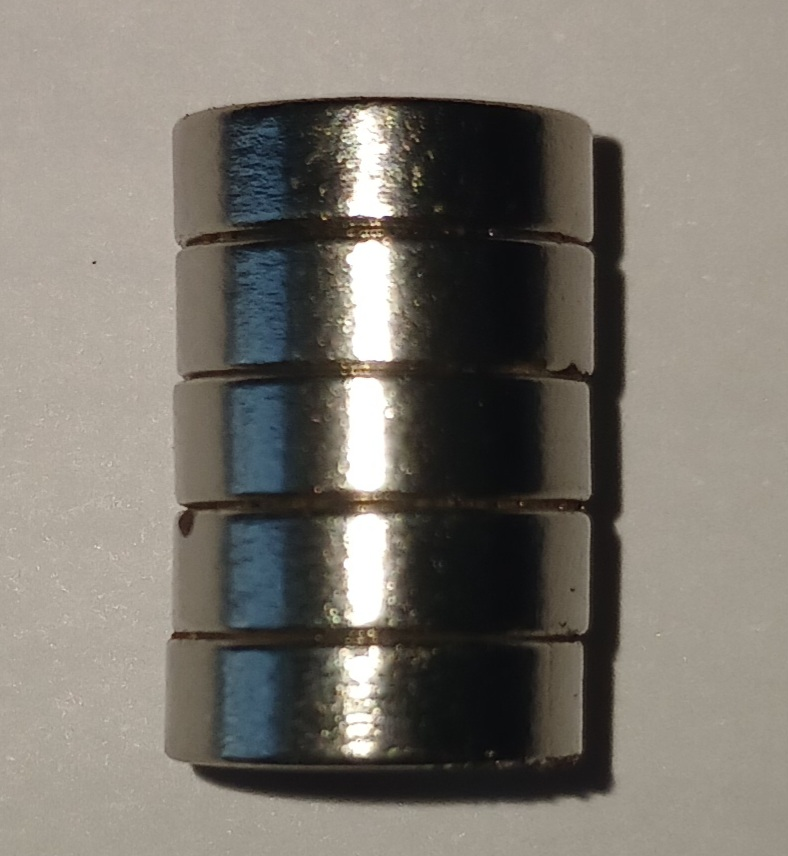
\includegraphics[height = 0.2\textheight]{figures/magnets.jpg}
		\caption{Cylindrical neodymium magnet}
		\label{fig:magnets}
	\end{subfigure}
	\begin{subfigure}[c]{0.4\textwidth}
		\centering
		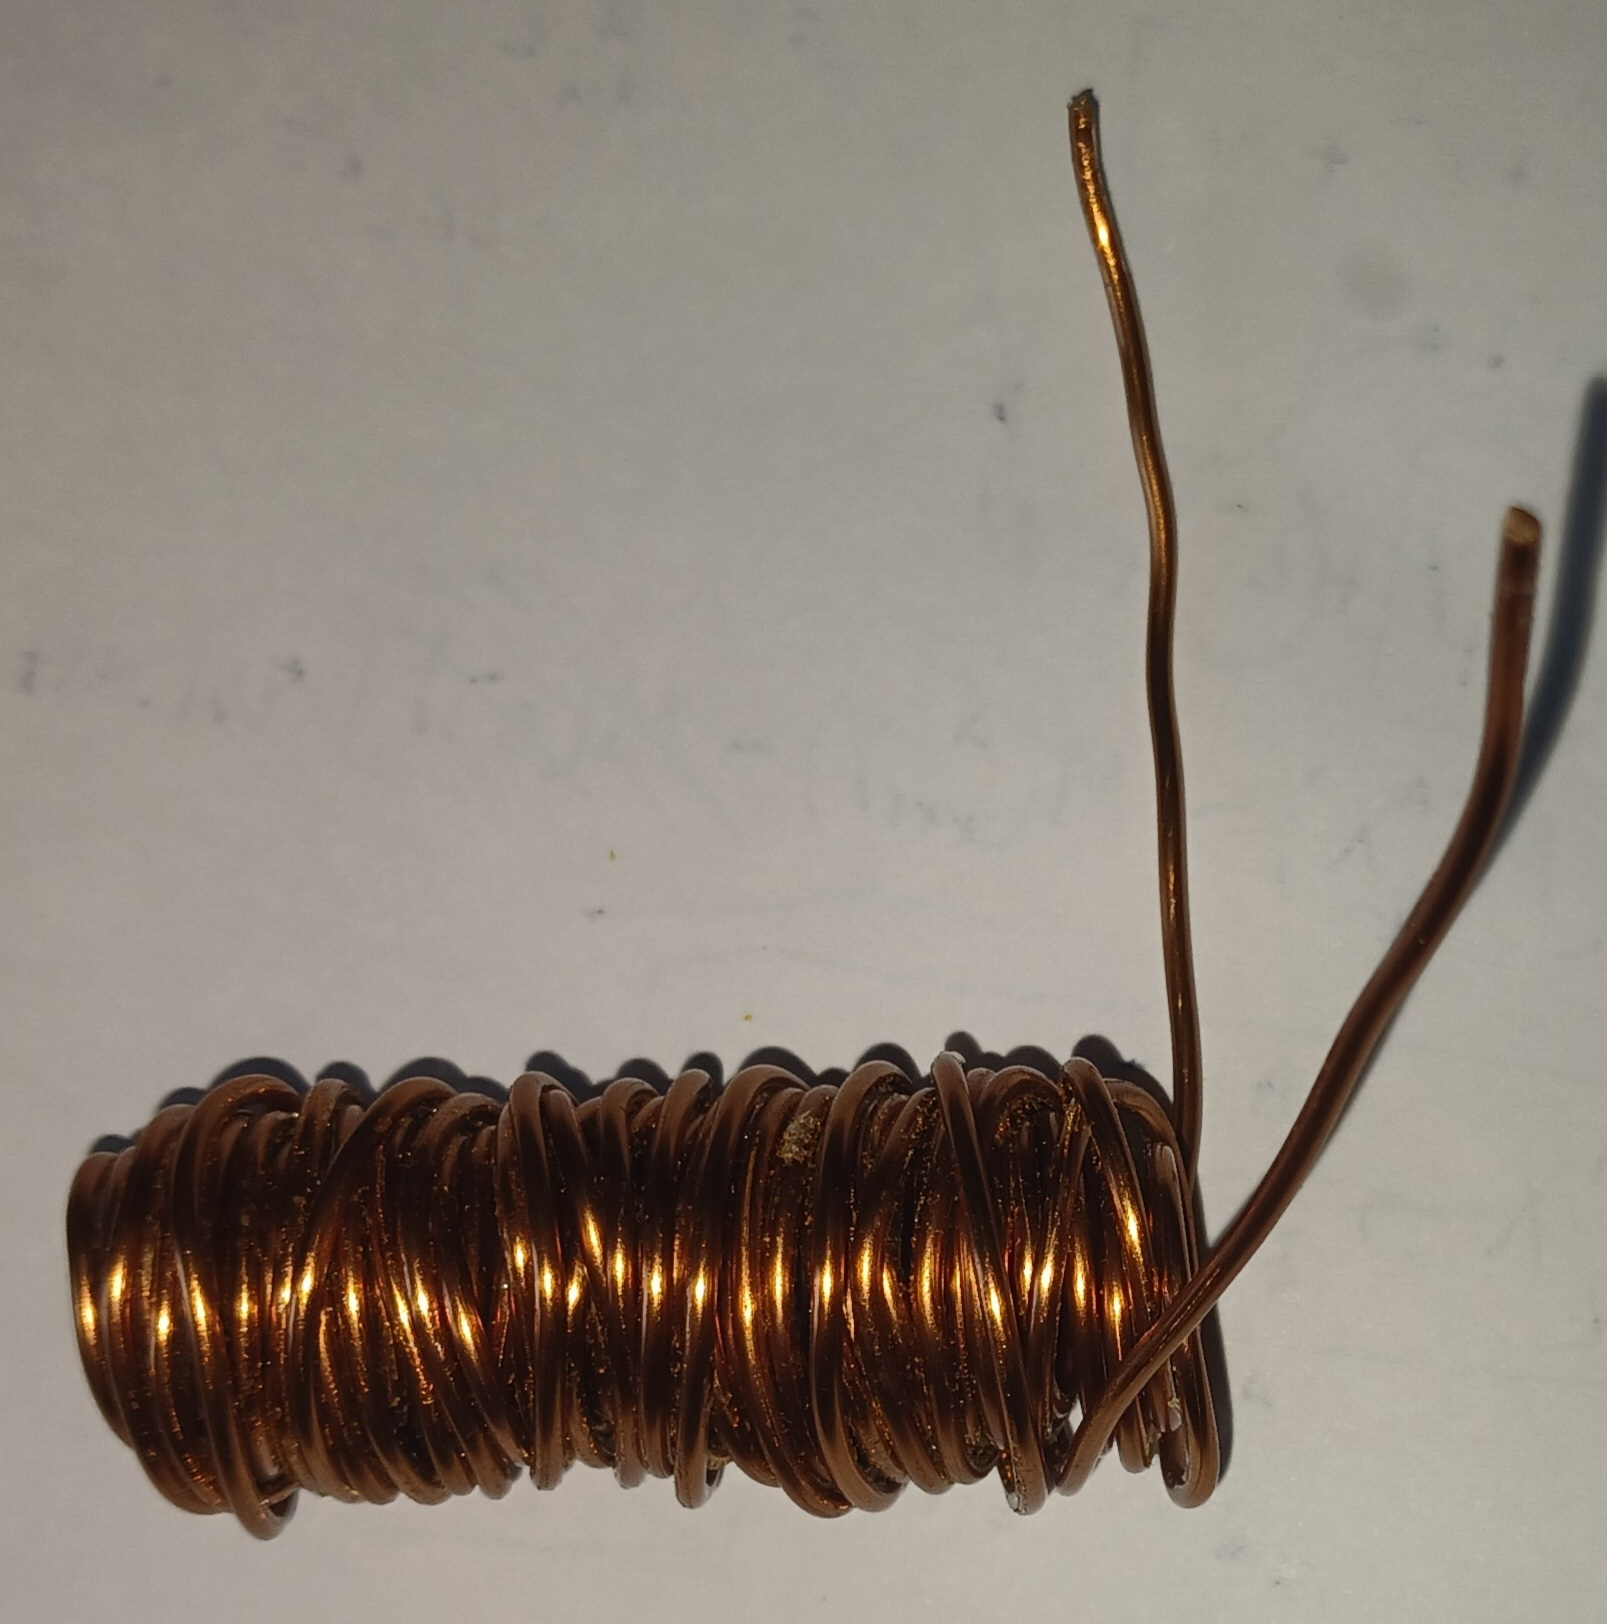
\includegraphics[height = 0.2\textheight]{figures/solenoid.jpg}
		\caption{Solenoid}
		\label{fig:solenoid}
	\end{subfigure}
	\caption{Materials used}
\end{figure}

\section{Methods}

\begin{enumerate}[noitemsep]
	\item Connect the solenoid to the oscilloscope.
	\item Place a piece of cloth below the solenoid.
	\item Hold the solenoid with the other piece of cloth $\qty{10}{\centi\meter}$ above the ground to prevent noise.
	\item Drop the magnets through the middle of the solenoid with varying heights from $\qty{0}{\centi\meter}$ to $\qty{14}{\centi\meter}$.
	\item Repeat five times for each height.
	\item Record the peak to peak voltage difference (Pk-Pk) from the oscilloscope.
\end{enumerate}

\section{Data analysis}
\label{sec:data-analysis}

The peak to peak voltage difference will be recorded onto a table, then plotted compared to the simulations.

To process the data and actually arrive at the gravitational acceleration, the Euler's method is used to simulate the dropping motion of the magnets with contributions from the Lenz law. Then, the position and velocity information is used to calculate the theoretical voltage. The code goes through every initial height in the range of $\qty{0}{\centi\meter}$ to $\qty{14}{\centi\meter}$ and gravitational acceleration values from $\qty{6}{\meter\per\second^2}$ to $\qty{12}{\meter\per\second^2}$. It then compares the theoretical result to the observed result and output the Earth's gravitational acceleration based on the minimum least mean squared error.

\begin{minted}{julia}
using Plots; plotlyjs()
using CUDA
using Statistics
using StatsBase
using Flux
# Variables declaration
global magneticPermeability = 1.256 * 10e-6
global solenoidLoopCount = 74
global solenoidRadius = 0.0058
global copperRadius = 0.00065
global solenoidLength = 2*π*solenoidRadius*solenoidLoopCount
global solenoidResistance = 1.68 * 10e-8 * solenoidLength
global copperDensity = 8850
global solenoidMass = solenoidLength * π * copperRadius^2 * copperDensity # 0.018
global magneticMoment = 0.4
global functionConst = (magneticMoment * magneticPermeability / 2)^2 * (12 * solenoidLoopCount * solenoidRadius) / (solenoidResistance * solenoidMass)
F(z) = functionConst * (2*z^3/(solenoidRadius^2 + z^2)^5 + z/(solenoidRadius^2 + z^2)^4)
# Voltage as a function of position of magnet and velocity
voltage(z, v) = @. - solenoidLoopCount * magneticPermeability * solenoidMass * z / 2 * v * (1/(solenoidRadius + z^2)^(3/2) - 3*z^2/(solenoidRadius^2 + z^2)^(5/2))

# Simulation configuration
global simTime = 0.4
global timeStep = 0.001
global timeInterval = CuArray(collect(0:timeStep:simTime))

# Simulating the voltage over time using Euler's method
function voltSim(initZ, gravitationalConst)
    posHistory = Float64.([initZ])
    veloHistory = Float64.([0.0])
    accel = - gravitationalConst
    for i in timeIndex #accel = - gravitationalConst + F(posHistory[i]) * veloHistory[i]
        nextVelo = veloHistory[i] + accel * timeStep
        push!(veloHistory, nextVelo)
        nextPos = posHistory[i] + veloHistory[i + 1] * timeStep
        push!(posHistory, nextPos)
    end
    minVoltage, maxVoltage = extrema(voltage.(posHistory, veloHistory))
    return abs(maxVoltage - minVoltage) # Return the predicted Pk-Pk output.
end

gVect = collect(9.52:0.00001:9.54)
zVect = collect(0:0.02:0.14)
gMat = gVect * ones(size(zVect, 1))'
zMat = ones(size(gMat, 1)) * zVect'

voltMat = voltSim.(zMat, gMat)
voltMatNorm = voltMat #.- minimum(voltMat, dims = 2)

data = [ # Raw data
    0.106  0.133  0.159  0.133  0.142;
    0.240  0.213  0.293  0.293  0.275;
    0.355  0.382  0.364  0.400  0.355;
    0.480  0.578  0.444  0.471  0.498;
    0.622  0.631  0.604  0.693  0.676;
    0.684  0.667  0.684  0.676  0.711;
    0.738  0.747  0.863  0.720  0.774;
    0.916  0.871  0.800  0.925  0.925;
] # Raw data, in millivolts
meanData = mean(data, dims = 2)

# Setup comparison
gVect = collect(6:0.00001:12)
zVect = collect(0:0.02:0.14)
gMat = gVect * ones(size(zVect, 1))'
zMat = ones(size(gMat, 1)) * zVect'
voltMat = voltSim.(zMat, gMat)

# Calculating errors
errorVect = []
rSqVect = []
# Error calculation
function rSquared(y, ypred)
    ss_res = sum((y .- ypred).^2)
    ss_tot = sum((y .- mean(y)).^2)
    return 1 - ss_res/ss_tot
end
for i in 1:size(gVect, 1)
    push!(errorVect, Flux.Losses.mse(normDat, voltMat'[:, i]))
    push!(rSqVect, rSquared(normDat, voltMat'[:, i]))
end
# Displaying the gravity
display(gVect[findall(x -> x == minimum(errorVect), errorVect)])
\end{minted}

\chapter{Results and discussion}

The data observed from five trials over eight initial height from $\qty{0}{\centi\meter}$ to $\qty{14}{\centi\meter}$ is listed in \cref{tab:raw-data} and plotted in \cref{fig:raw-data-with-mean}.
\begin{table}[ht]
	\centering
	\begin{tabular}{| C | C | C | C | C | C | C |}
		\hline
		\textrm{Initial height} & \multicolumn{5}{|c|}{\textrm{Pk-Pk voltage difference} (\unit{\volt})} & \textrm{Mean} \\
		\hline
		\qty{0}{\centi\meter} & 0.106 & 0.133 & 0.159 & 0.133 & 0.142 & 0.112 \\
		\qty{2}{\centi\meter} & 0.240 & 0.213 & 0.293 & 0.293 & 0.275 & 0.240 \\
		\qty{4}{\centi\meter} & 0.355 & 0.382 & 0.364 & 0.400 & 0.355 & 0.349 \\
		\qty{6}{\centi\meter} & 0.480 & 0.578 & 0.444 & 0.471 & 0.498 & 0.471 \\
		\qty{8}{\centi\meter} & 0.622 & 0.631 & 0.604 & 0.693 & 0.676 & 0.623 \\
		\qty{10}{\centi\meter} & 0.684 & 0.667 & 0.684 & 0.676 & 0.711 & 0.662 \\
		\qty{12}{\centi\meter} & 0.738 & 0.747 & 0.863 & 0.720 & 0.774 & 0.746 \\
		\qty{14}{\centi\meter} & 0.916 & 0.871 & 0.800 & 0.925 & 0.925 & 0.865 \\
		\hline
	\end{tabular}
	\caption{Observed Pk-Pk voltage difference}
	\label{tab:raw-data}
\end{table}

\begin{figure}[ht]
	\centering
	\includesvg[inkscapelatex = false, scale = 0.8]{raw-data.svg}
	\caption{Pk-Pk voltage difference plot from different trials with the mean value shown in black.}
	\label{fig:raw-data-with-mean}
\end{figure}

\Cref{fig:raw-data-with-mean} shows the observed data with the mean values from the five trials plotted in black. As seen, the mean values increases almost linearly with the initial height of the magnet. When the observation is plotted against the theoretical Pk-Pk voltage difference got from the simulation, the observation nearly lines up with the line $g = \qty{9.78}{\meter\per\second^2}$ shown in blue, which is Thailand's actual gravitational acceleration.

\begin{figure}[ht]
	\centering
	\includesvg[inkscapelatex = false, scale = 0.8]{theoretical-pk-pk.svg}
	\caption{Theoretical Pk-Pk voltage difference from $g = \qty{6}{\meter\per\second^2}$ to $\qty{12}{\meter\per\second^2}$ shown in colored lines. The blue line shows the theoretical Pk-Pk voltage difference of Thailand's actual gravity ($g = \qty{9.78}{\meter\per\second^2}$), and the black line shows the observed data.}
	\label{fig:theoretical-pk-pk}
\end{figure}
\begin{figure}[ht]
	\centering
	\includesvg[inkscapelatex = false, scale = 0.8]{mse-gravity.svg}
	\caption{The mean squared error between the theoretical Pk-Pk voltage difference and the observed voltage difference at different gravitaional acceleration values from $g = \qty{6}{\meter\per\second}$ to $g = \qty{12}{\meter\per\second}$. The blue dot shows the point where the mean squared error is lowest.}
	\label{fig:mse-gravity}
\end{figure}

The mean squared error between all the predicted Pk-Pk voltage difference and the observed voltage difference are then calculated and plotted in \cref{fig:mse-gravity}. The point where the error is the lowest is at $g = \qty{9.529}{\meter\per\second^2}$ with coefficient of determination, $R^2$ equals to $0.942$, showing that the observed data do correlates with the predicted Pk-Pk voltage difference.


\chapter{Conclusion}

In conclusion, we successfully demonstrated that the measurement of Earth's gravitational acceleration using a simple setup involving a free-falling magnet and a solenoid, analyzed through electromagnetic induction principles, is possible. The results indicated quite a strong correlation between the observed peak-to-peak voltage differences and the theoretical predictions, particularly aligning with the gravitational acceleration value of $\qty{9.529}{\meter\per\second^2}$, which is very close to Thailand's actual gravitational acceleration, which is around $\qty{9.78}{\meter\per\second^2}$.

However, it is important to note that the measured gravitational acceleration was slightly lower than the expected value. This discrepancy can be attributed to the experimental setup, specifically the lack of a guiding tube for the magnet. Without a tube, the magnet may have experienced slight collisions with the solenoid during its fall, which could have reduced the velocity of the magnet; thus, reducing the induced voltage also. Such interactions may have dampened the effectiveness of the electromagnetic induction process, leading to an underestimation of the gravitational force acting on the magnet.

Despite these challenges, the experiment validated the hypothesis that gravitational acceleration can be measured through induced voltage and highlighted the effectiveness of using basic materials and methods to achieve this goal. Future work could focus on refining the data processing methods and incorporating a guiding tube to minimize collisions, thereby enhancing the accuracy of gravitational measurements. Overall, this research underscores the potential of electromagnetic induction as a practical tool for measuring fundamental physical constants.

\newpage


% Bibliography
\printbibliography

\end{document}
